% Options for packages loaded elsewhere
\PassOptionsToPackage{unicode}{hyperref}
\PassOptionsToPackage{hyphens}{url}
%
\documentclass[
  oneside]{memoire-umons}
\usepackage{amsmath,amssymb}
\usepackage{iftex}
\ifPDFTeX
  \usepackage[T1]{fontenc}
  \usepackage[utf8]{inputenc}
  \usepackage{textcomp} % provide euro and other symbols
\else % if luatex or xetex
  \usepackage{unicode-math} % this also loads fontspec
  \defaultfontfeatures{Scale=MatchLowercase}
  \defaultfontfeatures[\rmfamily]{Ligatures=TeX,Scale=1}
\fi
\usepackage{lmodern}
\ifPDFTeX\else
  % xetex/luatex font selection
\fi
% Use upquote if available, for straight quotes in verbatim environments
\IfFileExists{upquote.sty}{\usepackage{upquote}}{}
\IfFileExists{microtype.sty}{% use microtype if available
  \usepackage[]{microtype}
  \UseMicrotypeSet[protrusion]{basicmath} % disable protrusion for tt fonts
}{}
\makeatletter
\@ifundefined{KOMAClassName}{% if non-KOMA class
  \IfFileExists{parskip.sty}{%
    \usepackage{parskip}
  }{% else
    \setlength{\parindent}{0pt}
    \setlength{\parskip}{6pt plus 2pt minus 1pt}}
}{% if KOMA class
  \KOMAoptions{parskip=half}}
\makeatother
\usepackage{xcolor}
\usepackage{graphicx}
\makeatletter
\def\maxwidth{\ifdim\Gin@nat@width>\linewidth\linewidth\else\Gin@nat@width\fi}
\def\maxheight{\ifdim\Gin@nat@height>\textheight\textheight\else\Gin@nat@height\fi}
\makeatother
% Scale images if necessary, so that they will not overflow the page
% margins by default, and it is still possible to overwrite the defaults
% using explicit options in \includegraphics[width, height, ...]{}
\setkeys{Gin}{width=\maxwidth,height=\maxheight,keepaspectratio}
% Set default figure placement to htbp
\makeatletter
\def\fps@figure{htbp}
\makeatother
\setlength{\emergencystretch}{3em} % prevent overfull lines
\providecommand{\tightlist}{%
  \setlength{\itemsep}{0pt}\setlength{\parskip}{0pt}}
\setcounter{secnumdepth}{-\maxdimen} % remove section numbering
\usepackage{algpseudocode}
\ifLuaTeX
  \usepackage{selnolig}  % disable illegal ligatures
\fi
\usepackage[]{biblatex}
\addbibresource{src/memoire-umons/ref.bib}
\IfFileExists{bookmark.sty}{\usepackage{bookmark}}{\usepackage{hyperref}}
\IfFileExists{xurl.sty}{\usepackage{xurl}}{} % add URL line breaks if available
\urlstyle{same}
\hypersetup{
  pdftitle={DBSCAN},
  pdfauthor={Bal Sébastien},
  hidelinks,
  pdfcreator={LaTeX via pandoc}}

\title{DBSCAN}
\usepackage{etoolbox}
\makeatletter
\providecommand{\subtitle}[1]{
  \apptocmd{\@title}{\\{\large #1}}{}{}
}
\makeatother
\subtitle{Lecture et rédaction scientifiques}
\author{Bal Sébastien}
\date{2022-2023}

\date{2022-2023}

\departement{informatics}


\service{Master Sciences Informatique}

\directeur{Mr Ben Thaieb}


\usepackage{bm}
% From https://github.com/Wandmalfarbe/pandoc-latex-template/blob/master/eisvogel.tex
\usepackage[headsepline,footsepline]{scrlayer-scrpage}
\newpairofpagestyles{umons}{
  \clearpairofpagestyles
  \ihead*{DBSCAN}
  \chead*{}
  \ohead*{2022-2023}
  \ifoot*{Bal Sébastien}
  \cfoot*{}
  \ofoot*{\thepage}
  \addtokomafont{pageheadfoot}{\upshape}
}
\pagestyle{umons}

%
% blockquote
%
\definecolor{blockquote-border}{RGB}{221,221,221}
\definecolor{blockquote-text}{RGB}{119,119,119}
\usepackage{mdframed}
\newmdenv[rightline=false,bottomline=false,topline=false,linewidth=3pt,linecolor=blockquote-border,skipabove=\parskip]{customblockquote}
\renewenvironment{quote}{\begin{customblockquote}\list{}{\rightmargin=0em\leftmargin=0em}%
\item\relax\color{blockquote-text}\ttfamily\ignorespaces}{\unskip\unskip\endlist\end{customblockquote}}

\begin{document}
\maketitle

{
\setcounter{tocdepth}{3}
\tableofcontents
}
\chapter{Introduction}

La détection de clusters est une tâche fondamentale en fouille de
données, permettant d'identifier des regroupements significatifs dans un
ensemble de données. Parmi les nombreux algorithmes de clustering,
DBSCAN (Density-Based Spatial Clustering of Applications with Noise)
s'est avéré être une approche puissante et largement utilisée. Dans cet
article, nous examinons en détail DBSCAN, en nous concentrant sur ses
concepts clés, son fonctionnement et sa performance. De plus, nous
effectuons une comparaison approfondie entre DBSCAN et CLARANS, un autre
algorithme de clustering, afin d'évaluer leur efficacité respective.

Avant de plonger dans les détails de DBSCAN, il est important de
comprendre certaines notions de base liées au clustering. Nous explorons
les concepts de densité, de voisinage et de bruit, qui sont des éléments
essentiels dans la méthode DBSCAN. Ces notions fournissent le fondement
nécessaire pour comprendre la logique sous-jacente de l'algorithme et
ses performances.

DBSCAN est un algorithme de clustering basé sur la densité, qui permet
d'identifier des clusters de formes arbitraires dans un espace de
données multidimensionnel. En utilisant des mesures de densité locales,
telles que le nombre minimum de points (MinPts) et le rayon
d'atteignabilité (Eps), DBSCAN peut distinguer les points centraux des
points de frontière et du bruit. L'algorithme se caractérise par sa
capacité à détecter des clusters de différentes tailles et formes, tout
en étant résistant aux valeurs aberrantes.

Un aspect crucial lors de l'utilisation de DBSCAN est le choix approprié
des paramètres d'entrée, à savoir MinPts et Eps. Dans cet article, nous
abordons différentes approches et techniques pour sélectionner ces
paramètres de manière adéquate, en tenant compte des caractéristiques
des données et des objectifs spécifiques du clustering. Nous discutons
également des implications de ces choix sur les performances de DBSCAN.

Pour évaluer la performance de DBSCAN, nous le comparons à CLARANS, un
autre algorithme de clustering. Nous examinons les différences entre les
deux approches en termes d'efficacité, de précision et de robustesse
vis-à-vis des données bruitées. À travers des expériences et des mesures
quantitatives, nous mettons en évidence les avantages et les limitations
de chaque algorithme, offrant ainsi des informations précieuses pour les
chercheurs et les praticiens dans le domaine du clustering.

En combinant une présentation détaillée de DBSCAN, une discussion sur le
choix des paramètres d'entrée et une évaluation comparative avec
CLARANS, cet article vise à fournir une vision approfondie de
l'algorithme DBSCAN, de ses performances et de son utilité dans
différentes applications de clustering.

\chapter{Les bases et notion de vocabulaire}

Dans ce chapitre, nous allons mettre les bases de la clusterisation et
les notions de vocabulaire pour la bonne compréhension de la suite de
l'article.

\hypertarget{base-de-donnuxe9es-spatiale}{%
\subsubsection{Base de données
Spatiale}\label{base-de-donnuxe9es-spatiale}}

Ce terme est associé à la gestion d'ensembles d'objets dans l'espace
plutôt qu'à des images ou des représentations graphiques de l'espace.
Elle permet de stocker des informations dans l'espace telle que des
bâtiments, des routes et des montagnes.

\hypertarget{cluster}{%
\subsubsection{Cluster}\label{cluster}}

Un cluster est un ensemble qui contient des points de données
similaires. Ces données sont regroupées suivant des critères définis par
l'algorithme de clustering.

\hypertarget{densituxe9}{%
\subsubsection{Densité}\label{densituxe9}}

Une densité est une mesure de la compacité des points de données dans un
cluster.

\hypertarget{algorithmes-de-regroupements}{%
\subsubsection{Algorithmes de
regroupements}\label{algorithmes-de-regroupements}}

Les algorithmes de regroupement, tels que définit par Kaufman et
Rousseeuw en 1990\footfullcite{kaufman1990finding}, se divisent en deux
catégories : les algorithmes de partitionnement et les algorithmes
hiérarchiques.

Un algorithme de partitionnement cherche à diviser une base de données D
en n objets en un ensemble de k clusters, dans lequel k est un paramètre
d'entrée fixé à l'avance. Comme première étape, l'algorithme de
partitionnement va créé une partion initiale à partir de la base de
données D, pour l'utiliser dans une méthode itérative afin d'optimiser
une fonction objective. Dans ces algorithmes, chaque cluster est
représenté soit par le centre de gravité du cluster comme le fait très
bien k-means, soit par l'un des objets du cluster situé près de son
centre comme k-medoid. Cette méthode en deux étapes faites par ces
algorithmes permet de déterminer dans un premier temps k qui minimise la
fonction objective, ensuite à attribuer à chaque objet du cluster dont
le représentant est le plus proche de lui.

Un algorithme hiérarchique permet de créer une décomposition
hiérarchique de la base de données D. Celle-ci est représentée par un
dendogramme, qui est un arbre divisant itérativement D en sous-ensemble
plus petits jusqu'à ce que chaque sous-ensemble ne contienne plus qu'un
seul objet. Chaque noeud de l'arbre représente un cluster de D. Le
dendogramme peut être construit de deux manières différentes : soit en
partant des feuilles pour arriver à la racine (approche agglomérative),
soit en partant de la racine pour arriver aux feuilles (approche
divisive), en fusionnant ou divisant les clusters à chaque étape.

Contrairement aux algorithmes de partitionnement, les algorithmes
hiérarchiques ne nécessitent pas de paramètre d'entrée k. Par contre,
une condition d'arrêt doit être définie pour indiquer quand le processus
de fusion ou de division doit s'arrêter.

\hypertarget{k-means}{%
\subsubsection{K-Means}\label{k-means}}

L'algorithme K-Means vise à regrouper un ensemble de données en un
certain nombre de clusters pré-définis par l'utilisateur. Cette méthode
de clustering non hiérarchique commence en sélectionnant aléatoirement K
centres de clusters, puis chaque point de données est ensuite attribué
au centre du cluster le plus proche. Les centres des clusters sont
ensuite mis à jour en utilisant les points de données nouvellement
attribués et le processus se répète jusqu'à ce que les centres des
clusters convergent vers une solution stable ou que le nombre
d'itérations maximum soit atteint \footfullcite{tan2006introduction}.

\hypertarget{k-medoid}{%
\subsubsection{K-Medoid}\label{k-medoid}}

L'algorithme K-Medoid est une méthode de clustering qui vise à diviser
un ensemble de données en un nombre prédéfini de clusters. Il utilise
des objets réels de chaque cluster, ce qui rend l'algorithme plus
résistant aux valeurs aberrantes \footfullcite{bishop2006pattern}.
Celui-ci commence par sélectionner k objets de l'ensemble de données
comme médoides initiaux, qui sont les objets qui minimisent la distance
moyenne aux autres objets dans leur cluster. Ensuite, chaque objet est
assigné au medoide le plus proche et les medoides sont mis à jour en
choisissant le nouvel objet qui minimise la somme des distances entre
lui et tous les autres objets de son cluster. Le processus est répété
jusqu'à ce que les medoides ne changent plus ou que le nombre maximum
d'itérations soit atteint \footfullcite{han2011data}.

\hypertarget{clarans}{%
\subsubsection{CLARANS}\label{clarans}}

Ng et Han en 1994\footfullcite{ng1994efficient} ont exploré les
algorithmes de partitionnement pour l'extraction de connaissances à
partir de bases de données spatiales. Ils ont présenté une méthode
améliorée de K-Medoid appelée CLARANS (Clustering Large Application
based on RANdomized Search), qui est plus efficace et performante que
les anciennes méthodes de K-Medoid. Malheureusement, elle est très
coûteuse en temps et en exécution pour de grandes bases de données, car
elle implique des appels en \(\mathcal{O}(n)\). CLARANS suppose
également que tous les objets à regrouper peuvent résider en mémoire
principale en même temps, ce qui n'est pas toujours possible pour de
grandes bases de données.

\chapter{L'algorithme DBSCAN}

Nous allons parler dans ce chapitre de l'algorithme DBSCAN (Density
Based Spatial Clustering of Applications with Noise), celui-ci est conçu
pour détecter les clusters et le bruit dans une base de données
spatiale. Il permet d'identifier des points aberrants et de les écarter
de la solution finale.

L'idée la plus importante est le fait de prendre, pour chaque point d'un
cluster, un voisinage d'un rayon donné, celui-ci doit contenir au moins
un nombre minimum de points (MinPts), de sorte que la densité dans le
voisinage dépasse un seuil déterminé (Eps).

Pour que l'algorithme fonctionne correctement, il a besoin de prendre
deux paramètres en entrée. Ceux-ci sont MinPts, représenté par le nombre
minimum de points situé à une distance inférieure ou égale à Eps,
celui-ci est la distance qui permet de définir les points voisins d'un
point donné. Il peut bien entendu prendre quatre paramètres en entrée.
Dans l'article ``A Denity Based Algorithm for discovering clusters
\ldots{}''\footfullcite{ankerst1999optics}, les auteurs nous montrent
qu'ils utilisent quatre paramètres à l'algorithme, une liste de points
venant d'une base de données spatiale, la distance Eps pour définir les
voisins, un nombre minimum de points requis pour qu'un point soit
considéré comme central et que son voisinage soit dense, et une fonction
pour calculer la distance entre deux points.

DBSCAN permet de distinguer trois types de points, les points centraux,
les points frontières et les points aberrants. Les points centraux sont
ceux qui contiennent un voisinage dense, les points frontières sont ceux
qui font partie du voisinage d'un point central, et les point aberrants
ne sont ni centraux, ni frontières, ce sont des points de bruits.

Lorsque l'on applique l'algorithme de clustering DBSCAN à un ensemble de
données, les points centraux sont déterminés en fonction de leur
proximité avec d'autres points dans l'ensemble. Les points qui sont à
une distance inférieure ou égale à une valeur Eps sont regroupés
ensemble dans un même cluster, mais leur étiquette de cluster peut être
différente selon l'ordre dans lequel les clusters sont découverts. Les
points qui se trouvent à la frontière de plusieurs clusters différents
sont assignés au premier cluster découvert. Chaque cluster contient au
moins un point central, mais peut contenir moins de points si certains
des points centraux sont situés à une distance inférieure ou égale à Eps
de points situés à la frontière d'un autre cluster.
HDBSCAN\footfullcite{campello2013hdbscan} est un modèle amélioré qui
résout ce problème en éliminant la notion de point frontière. Ce modèle
est donc capable de produire des clusters plus homogènes et plus
cohérents.

\hypertarget{approche-mathuxe9matique-de-lalgorithme}{%
\subsection{Approche mathématique de
l'algorithme}\label{approche-mathuxe9matique-de-lalgorithme}}

L'article présente plusieurs définitions :

\textbf{Définition 1} (Voisinage Eps d'un point) :

Un voisinage Eps d'un point p, ce note \(N_{Eps}(p)\), avec un ensemble
d'objets D, \(N_{Eps}(p) = \{q \in D \mid distance(p,q) \leq Eps\}\)

Lorsque tous les points qui sont inférieurs ou égaux à Eps sont inclus
dans un même voisinage, il peut y avoir une confusion entre les
différents clusters. Pour éviter cette confusion, il est recommandé de
sélectionner un point central pour chaque cluster et de garantir que
tous les points dans ce cluster se trouvent dans le voisinage de Eps de
ce point central.

\textbf{Définition 2} (directemennt densité-atteignable)

Si un point q satisfait la condition de densité-atteignable directe par
rapport à Eps et MinPts depuis un point q, alors on peut dire que p est
directement densité-atteignable à partir de q.

Pour satisfaire les conditions, il faut que ça respecte ceci :

\begin{enumerate}
\def\labelenumi{\arabic{enumi}.}
\item
  \(p \in N_{Eps}(q)\)
\item
  \(\mid N_{Eps}(q)\mid \geq MinPts\)
\end{enumerate}

\textbf{Définition 3} (Densité-atteignable)

La densité-atteignable d'un point p par rapport à un point q en
utilisant Eps et MinPts est établie s'il existe une séquence de points
\(p_{1}\) à \(p_{n}\), telle que \(p_{1} = q\), \(p_{n} = p\) et que
chaque point \(P_{i+1}\) est directement densité-atteignable à partir de
\(P_{i}\).

Afin d'établir l'accessibilité entre deux points tels que p et q, il est
nécessaire qu'une séquence de points reliant p à q soit présente, et que
chaque point de cette séquence, soit densité-atteignable à partir du
précédent. De cette façon, p et q deviennent densités-atteignables à
partir d'autres points.

\textbf{Définition 4}(Densité-connecté)

Pour que deux points soient densités-connectés entre eux par rapport à
Eps et MinPts, il faut qu'il y ait un point o qui permette à la fois à p
et q d'être densité-atteignables par rapport à Eps et MinPts.

\textbf{Définition 5}(Cluster)

Un ensemble de points présent dans une base de données de points D. Un
cluster C par rapport à Eps et MinPts est un sous-ensemble non vide de D
qui répond aux conditions ci-dessous :

\begin{enumerate}
\def\labelenumi{\arabic{enumi}.}
\tightlist
\item
  \(\forall p,q\) : si \(p \in C\) et q est densité-atteignable depuis
  p, alors \(q \in C\)(Maximalité).
\item
  \(\forall p,q \in C :p\) est densité-connecté à q par rapport à Eps et
  MinPts(Connectivité).
\end{enumerate}

\textbf{Définition 6}(Bruit)

En partant de \(C_{1}, ...,C_{k}\) des clusters de l'ensemble de données
D par rapport à Eps et MinPts i, i=1,\ldots,k. On peut définir le bruit
comme un ensemble de points dans l'ensemble de données D ne faisant
partie d'aucun cluster \(C_{i}\), en d'autres mots,
\(\{p \in D \mid \forall i\) : \(p \notin C_{i}\}\)

Le seul moment où on peut être certain qu'un point est aberrant est que
son eps-voisinage ne contient qu'un seul point, lui même. Un point
aberrant est un point qui ne fait partie d'aucun cluster.

À présent, on peut s'occuper des lemmes, ceux-ci vont permettre de
définir le comportement de notre algorithme.

\textbf{Lemme 1}

Un point p dans D et \(\mid N_{Eps}(p)\mid \geq\) MinPts. Alors
l'ensemble \(\mathcal{O} = o \mid o \in D\) et o est densité-atteignable
depuis p par rapport à Eps et MinPts est un cluster par rapport à Eps et
MinPts.

Ce qui signifie que l'on construit le cluster en partant de p, puis en y
ajoutant tous les points qui sont à une densité-atteignable depuis p et
qui respectent les critères de distance Eps et de densité minimal
MinPts.

\textbf{Lemme 2}

Soit C un cluster par rapport à Eps et MinPts et p un point quelconque
dans C avec \(\mid N_{Eps}(p)\mid \geq MinPts\). Alors C est égal à
l'ensemble \(\mathcal{O} = \{o \mid o\) est densité-atteignable depuis p
par rapport à Eps et MinPts \(\}\).

Celui-ci permet de définir que chaque point peut récupérer tous les
points atteignables à partir de n'importe quel point central. Ce qui
signifie que le cluster contient tous les points qui sont distances
atteignables d'un point central\footfullcite{rezaei2015density}.

À partir des lemmes définis plus haut, la présentation de l'algorithme
va être possible :

Function DBSCAN (Points : Points{[}{]}, eps : float, minPts : int)

\begin{algorithmic}
\State $cluster \gets 1$
\For{$i = 1 \to Points.size$}
\State $point \gets Points[i]$
\If{$point.idCluster = Null$}
\State $voisins \gets rechercheV(point, Points,Eps)$
\If{$voisins.taille \geq minPts$}
\State $point.idCluster \gets cluster$
\State $etendreCluster(voisins,Points, cluster,eps, minPts)$
\State $cluster \gets cluster+1$
\Else
\State $point.cluster \gets 0$
\EndIf
\EndIf
\EndFor
\end{algorithmic}

Function etendreCluster(voisins : Points{[}{]}, points : Points{[}{]},
cluster : int, eps : int, minPts : int)

\begin{algorithmic}
\For {$point \to voisins$}
\If {$point.clu = NIL$}
\State $point.clu \gets cluster$
\State $voisinLocal \gets rechercheV(point, points, eps)$
\If {$voisinLocal.taille \geq minPts$}
\State $voisinLocal \gets voisins \cup voisinLocal$
\EndIf
\EndIf
\EndFor
\end{algorithmic}

L'algorithme commence par initialiser tous les points comme n'étant pas
classifiés. Par la suite, il prend chaque point non classé, vérifie s'il
est possible de former un cluster à partir de ce point en utilisant la
fonction ``etendreCluster''. S'il en est capable, alors il est nouveau
et est attribué identifiantCluster et l'algorithme continue à chercher
d'autres points pour le cluster qu'il vient de commencer à créer.

La fonction etendreCluster permet de récupérer tous les points dans un
voisinage à une distance Eps à partir du point actuel. Pour chaque point
dans le tableau des voisins, on vérifie si le point n'a pas déjà été
assigné à un cluster. S'il est non assigné(NIL), on lui attribue
l'identifiant du cluster en cours ``cluster''. Par la suite, on effectue
une recherche du voisinage autour de ce point en utilisant la fonction
rechercheV. Si le nombre de voisins trouvés est supérieur ou égal à
MinPts, on ajoute ces voisins au tableau des voisins explorés. Une fois
que tous les points du tableau ont été traités, la fonction se termine.

\chapter{Le bon choix des paramètres de DBSCAN}

\hypertarget{minpts}{%
\subsection{MinPts}\label{minpts}}

Le paramètre de MinPts, permet une qualité du cluster et de la
performance. Malheureusement, il n'y a pas de méthode universelle pour
la déterminer, c'est pourquoi cela dépend de la nature des données et
des objectifs de l'analyse. Il est important de bien définir la bonne
valeur pour minimiser le bruit.

Dans l'article ``ADBSCAN: Adaptive Density-based\ldots{}'', une approche
adaptive est faite pour utiliser une mesure de densité locale pour
estimer le nombre de voisins dans un rayon donné autour de chaque point.
Cette mesure de densité est utilisée pour calculer une valeur de MinPts
locale pour chaque point, qui est ensuite utilisée dans DBSCAN. Grâce à
cela, il est possible d'identifier avec succès des clusters avec des
densités variables dans différents ensembles de données.

\hypertarget{eps}{%
\subsection{Eps}\label{eps}}

Le paramètre de Eps, est aussi un choix délicat pour le bon
fonctionnement de DBSCAN. Ce paramètre est aussi important, si cette
mesure n'est pas bonne cela peut entrainer des regroupements incorrects
ou une division en plusieurs clusters.

Il y a plusieurs méthodes pour sélectionner la valeur de Eps, en
utilisant une base de données sur la densité, par essais erreurs ou pour
notre cas qui nous intéresse, en utilisant la méthode k-distance.
L'article de Ester et al.~\footfullcite{ester} propose une procédure qui
repose sur la notion de la fonction k-dist, celle-ci mesure la distance
entre chaque point d'une base de données et son k-ième voisin le plus
proche. Avec cette fonction, on construit un graphe qui fournit des
informations sur la densité des points et la présence de points
aberrants.

Afin de déterminer la valeur de Eps, on identifie le premier ``creux''
dans le graphe de la fonction k-dist. Ce creux correspond au point de
seuil où tous les points situés à sa gauche sont considérés comme
appartenant aux clusters dans la base de données.

Ainsi, en trouvant ce point de seuil, on définit la valeur d'Eps qui
sépare les points aberrants des points appartenant aux clusters dans la
base de données.

Dans l'article de Ester et al.~\footfullcite{ester}, on constate que la
valeur de k, une fois à 4, dans le graphe k-dist pour des données
bidimensionnelles ne change pas grandement. À partir, de la valeur k=3,
le graphe ne change que très peu, lui aussi. C'est pour cette raison,
qu'Ester et al.\footfullcite{ester} décident de garder par défaut la
valeur de k=4 pour MinPts pour calculer le graphe k-dist.

\begin{figure}
\centering
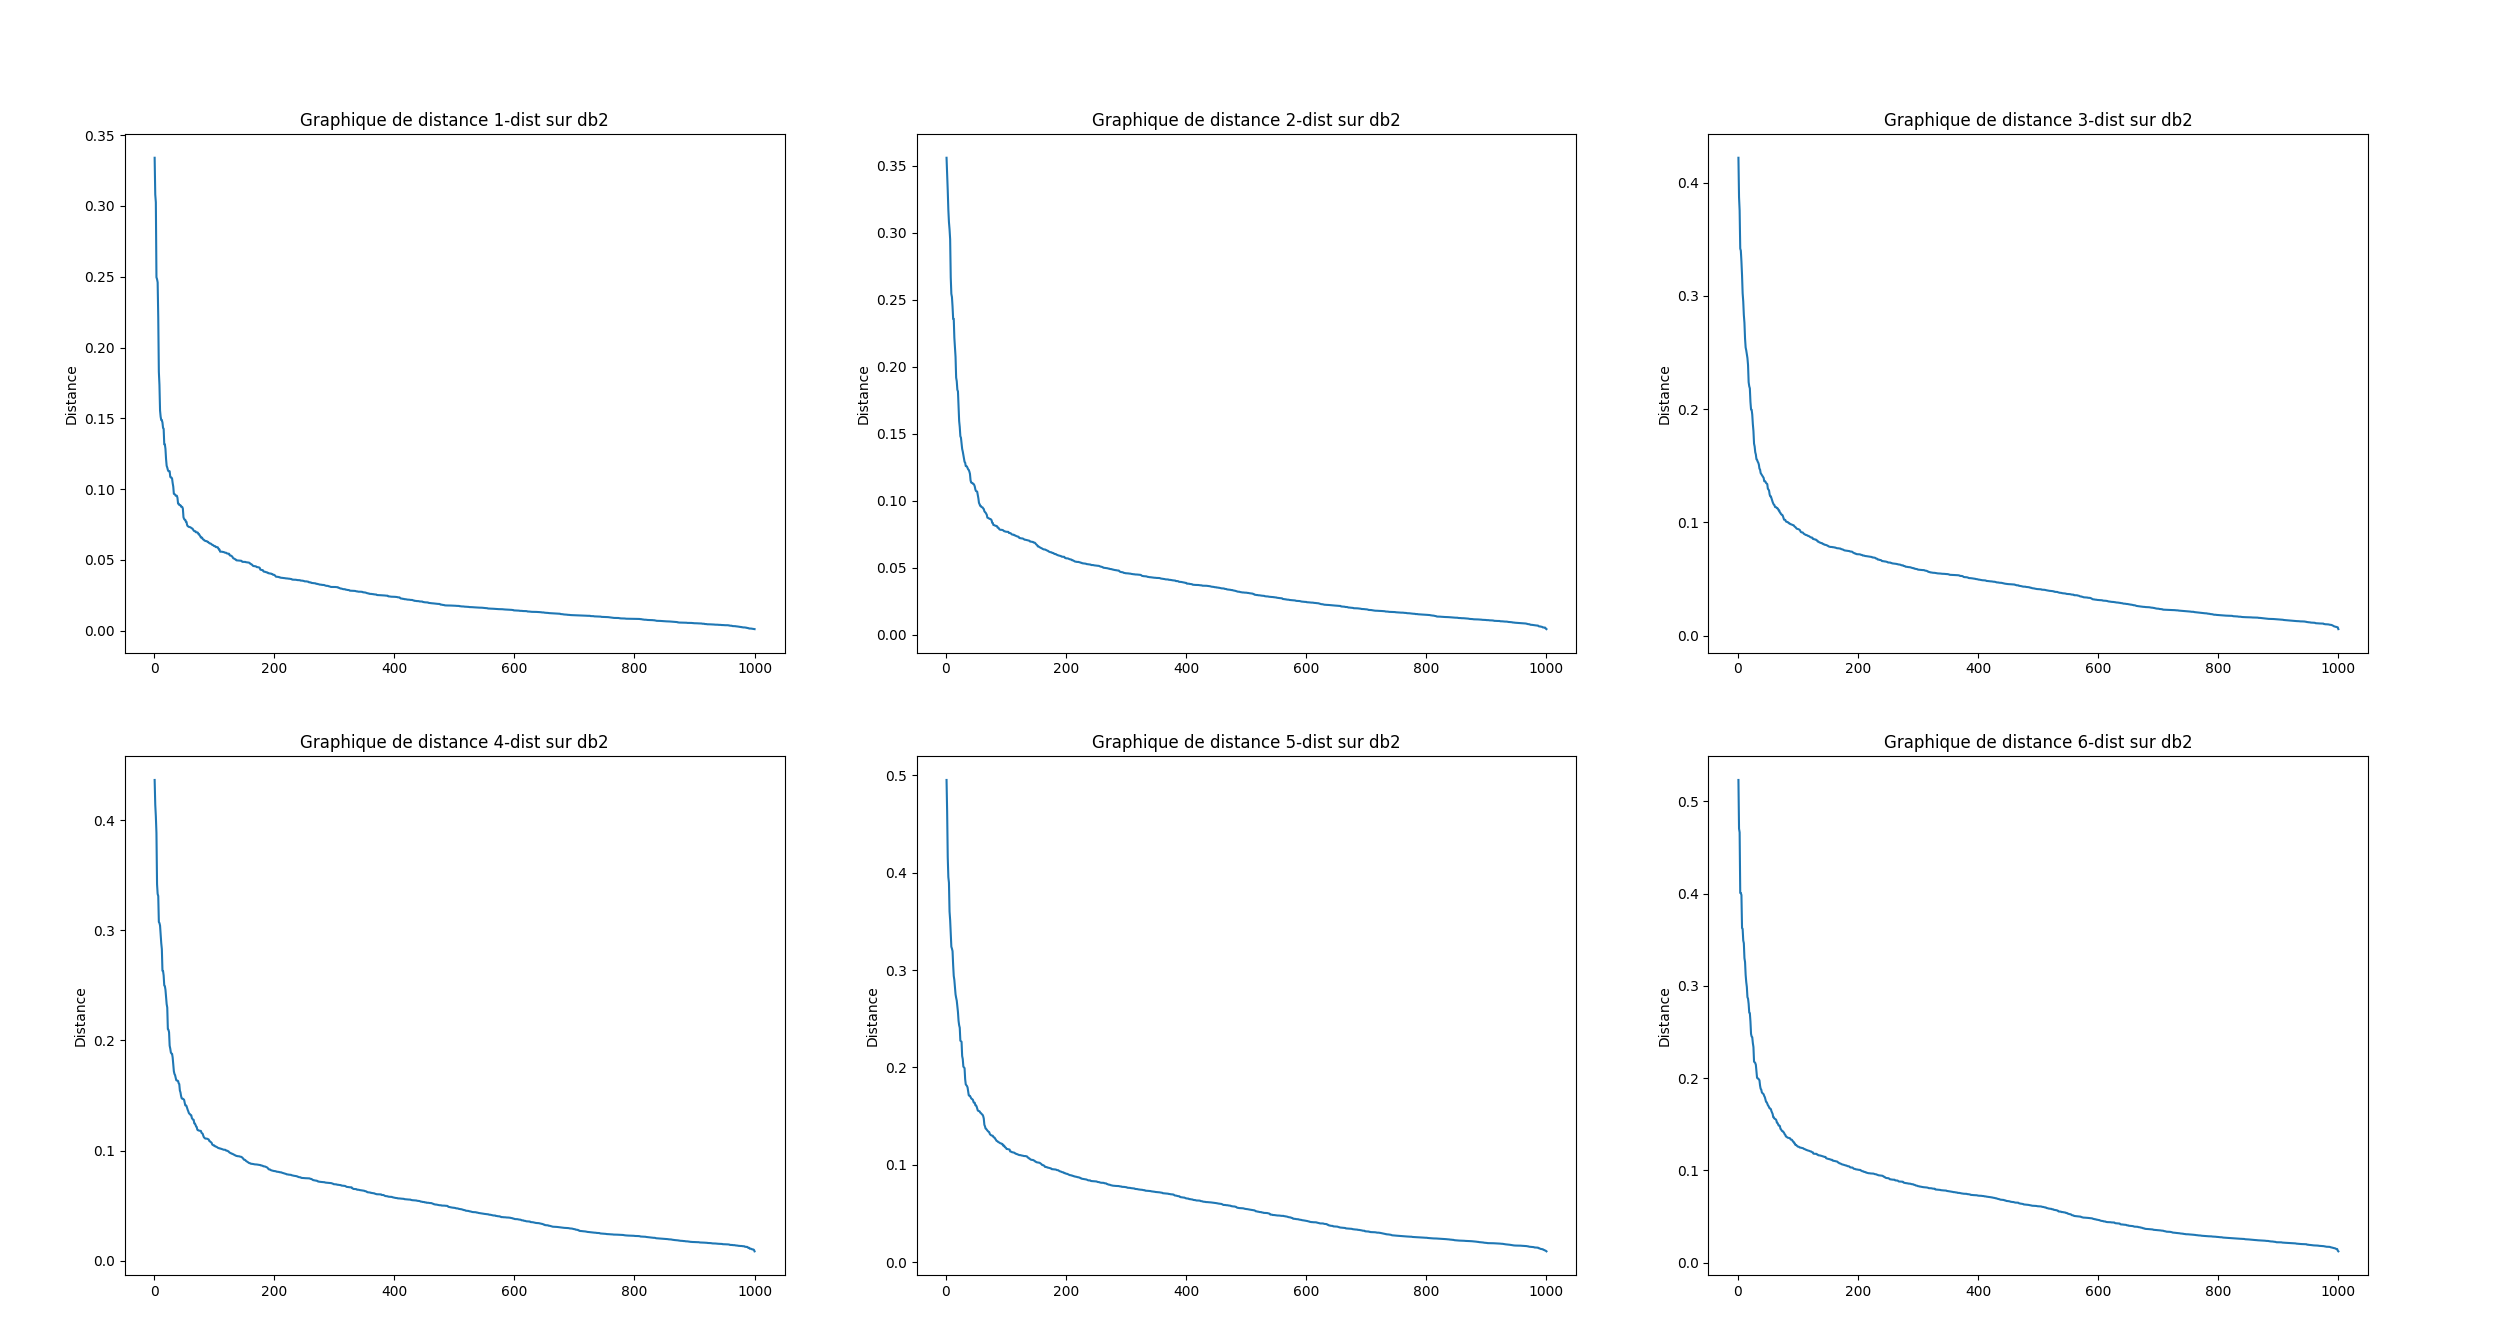
\includegraphics{src/memoire-umons/images/new_versions/k_dist_trie_db2.png}
\caption{Graphique k-dist du schéma 6 \label{k_dist}}
\end{figure}

\begin{figure}
\centering
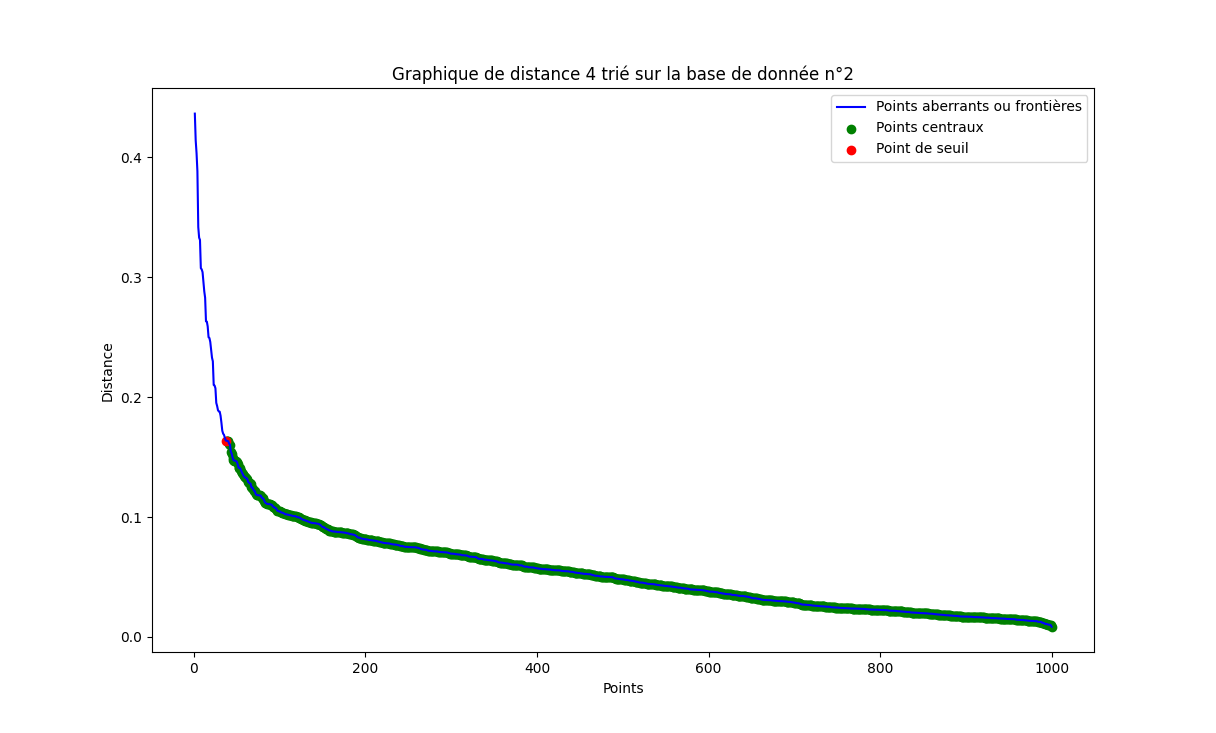
\includegraphics{src/memoire-umons/images/new_versions/k_dist_db2.png}
\caption{Graphique avec des données triées pour la db
\label{k_dist_trie}}
\end{figure}

\chapter{Performances}

\hypertarget{complexituxe9-de-la-fonction-recherchev}{%
\subsection{Complexité de la fonction
rechercheV}\label{complexituxe9-de-la-fonction-recherchev}}

Cette fonction utilisée dans l'algorithme de DBSCAN permet de rechercher
des voisins, celle-ci dépend généralement de l'algorithme d'accès
spatial utilisé pour organiser les données. En règle générale, ce sont
les arbres R*-trees qui sont utilisés pour accélérer la recherche des
voisins. Cette complexité montrée par Martin et
al.~\footfullcite{ester}, démontre que cette complexité est fréquemment
en \(\mathcal{O}(log (n + k))\), dans lequel n est le nombre total de
points dans la base de données et k le nombre moyen de voisins dans le
voisinage.

Dans leur article Ester et al.\footfullcite{ester} prétendent que leur
algorithme DBSCAN se termine en \(\mathcal{O}(n\cdot log (n))\).
Cependant il s'avère que cette affirmation est incorrecte, comme l'a
récemment souligné Gunawan\footfullcite{wang2013faster} l'algorithme de
(Ester)\footfullcite{ester} s'exécute en \(\mathcal{O}(n^2)\) dans le
pire des cas, indépendamment des paramètres Eps et MinPts.

\hypertarget{comparaison-entre-dbscan-et-clarans}{%
\subsection{Comparaison entre DBSCAN et
CLARANS}\label{comparaison-entre-dbscan-et-clarans}}

Dans cette partie, on va s'intéresser aux performances entre DBSCAN et
CLARANS, celui-ci était le premier et seul algorithme de regroupements
dans le but d'extraire des connaissances d'une base de données.

Comme CLARANS et DBSCAN sont deux algorithmes de regroupement distincts,
il n'existe pas de mesure quantitative commune permettant d'évaluer
précisément leur classification. L'évaluation faite ici est
principalement visuelle.

Une construction de différentes bases de données est utilisée pour
comparer visuellement l'exécution de DBSCAN avec celui de CLARANS. Les
données sont générées aléatoirement en suivant certains modèles, ceux-ci
vont permettre une meilleure visualisation des différents algorithmes.
Ils sont visibles sur la figure \ref{all_schemas}. Les divers modèles
générés ont puisé leur inspiration à partir des ressources disponibles
sur le site de scikit learn\footfullcite{scikit-learn-examples}. Cette
source a également servi de référence pour la création et l'exécution du
code visant à générer les divers schémas de regroupements.

\begin{figure}
\centering
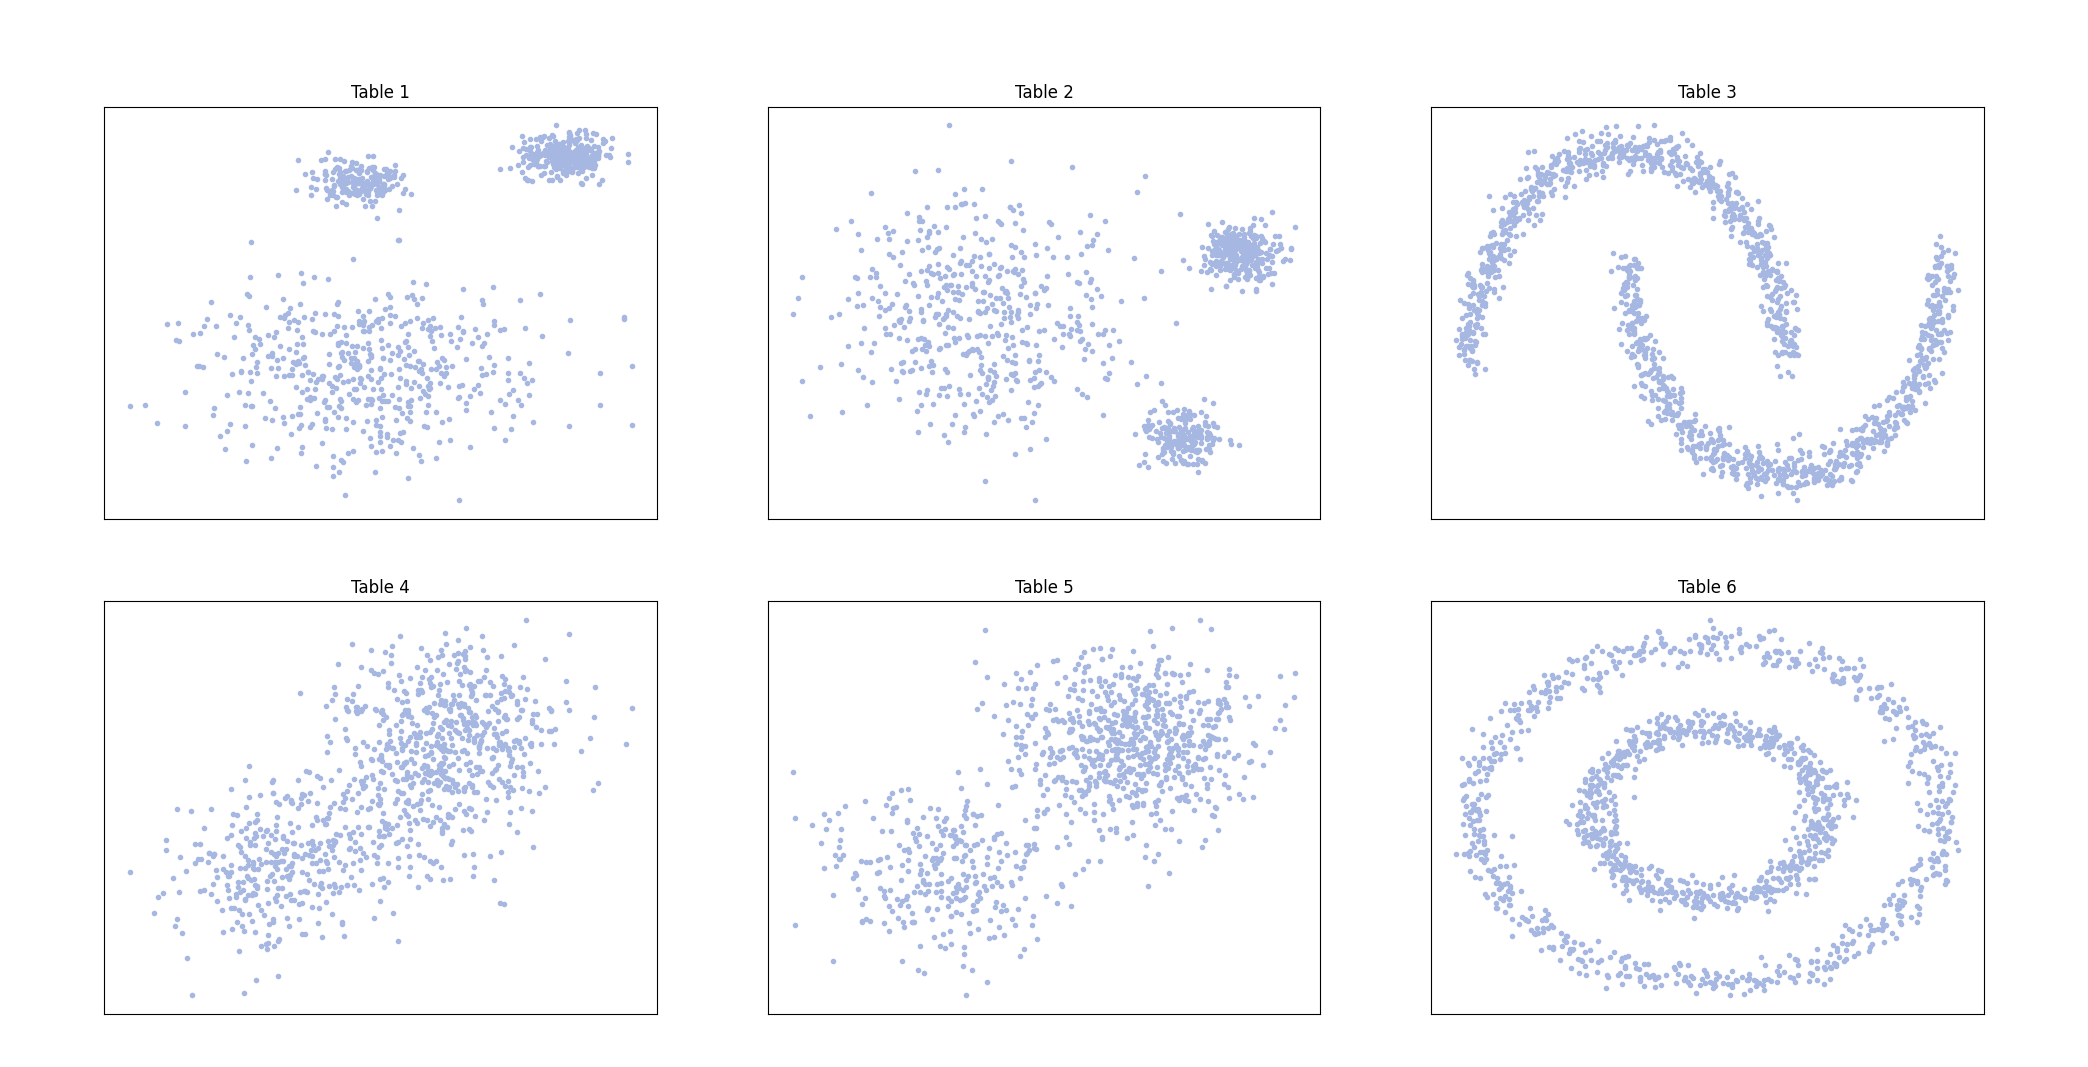
\includegraphics{src/memoire-umons/images/new_versions/clusters_all.png}
\caption{Différentes base de données \label{all_schemas}}
\end{figure}

Dans un premier temps, l'exécution de l'algorithme de CLARANS, le
paramètre k est choisit pour aider l'algorithme à trouver plus
facilement les différents clusters. Cela a était fait par essais erreurs
jusqu'au moment ou l'algorithme paraissait regrouper plusieurs clusters
visibles facilement à l'oeil. Nous pouvons remarquer le résultat sur la
figure \ref{clarans_all}.

\begin{figure}
\centering
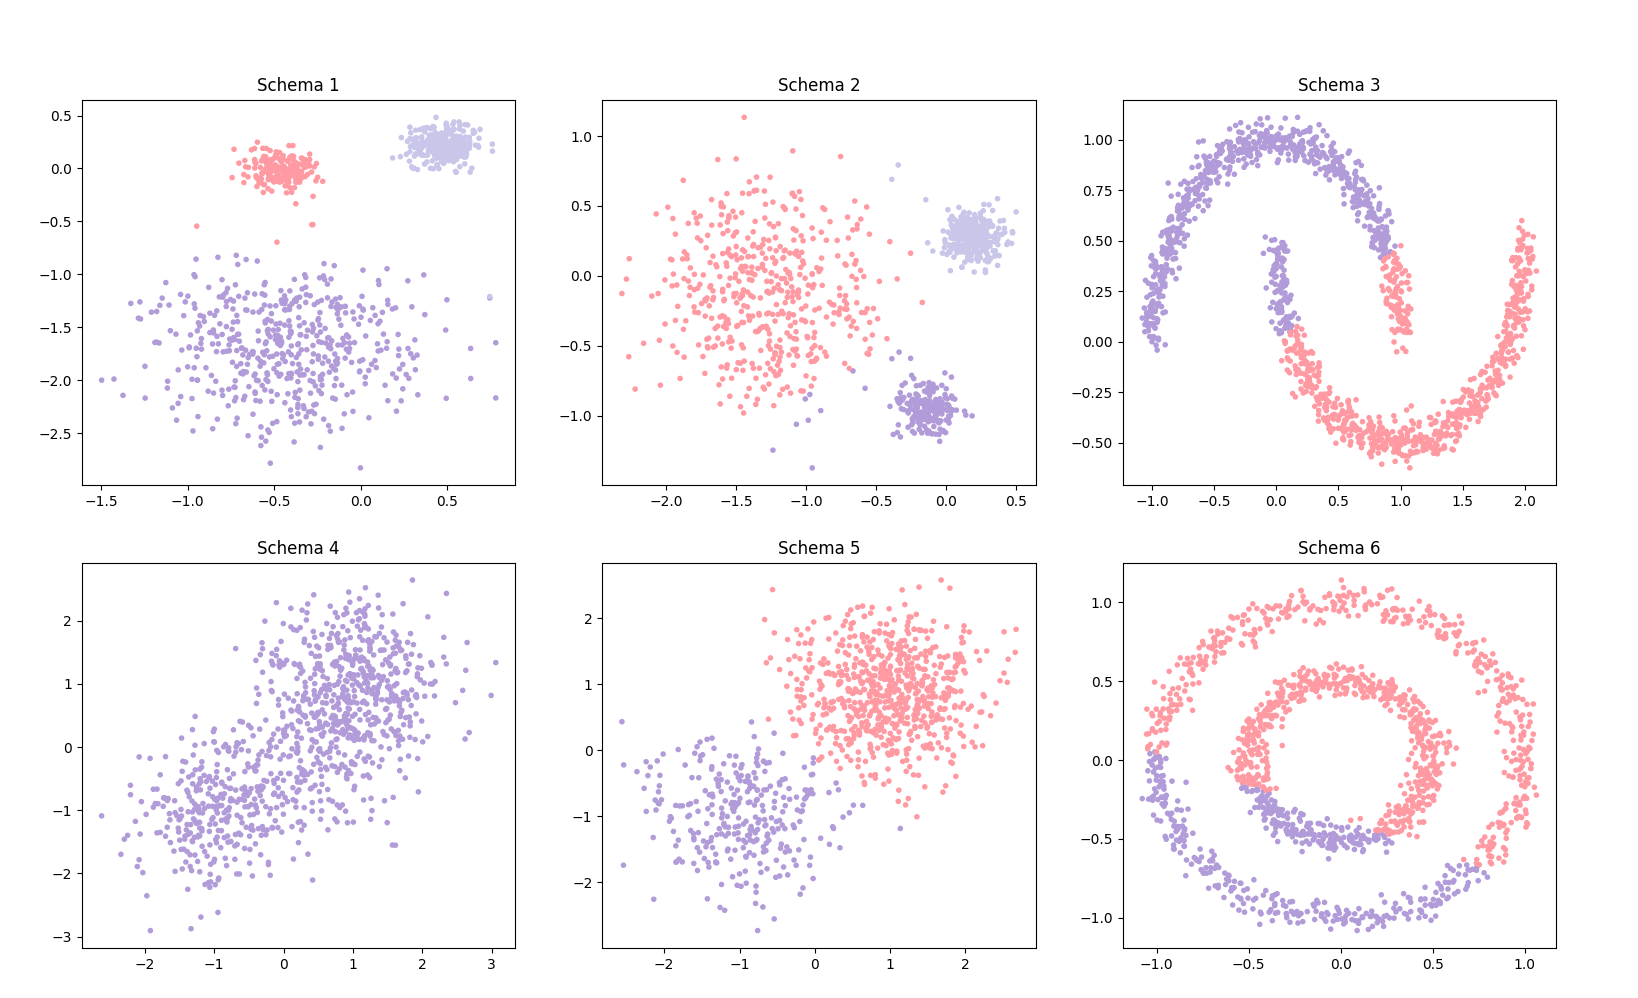
\includegraphics{src/memoire-umons/images/new_versions/clarans_all.png}
\caption{Résultats de CLARANS sur les bases de données
\label{clarans_all}}
\end{figure}

Dans les illustrations 1 et 2, il est évident que l'algorithme CLARANS
génère trois clusters bien définis. Cependant, il est important de noter
que le concept de bruit n'est pas pris en compte.

En examinant le schéma 3, la présence de deux quartiers de lune est
observable, et pourtant les résultats produits par CLARANS ne captent
pas correctement la structure des données, même si les points sont
proches les uns des autres.

En ce qui concerne le schéma 4, on observe que CLARANS inclut tous les
points dans des clusters, sans considérer les valeurs aberrantes qui
pourraient être présentes.

Dans le schéma 5, les performances de CLARANS sont meilleures puisqu'il
parvient à bien séparer les différentes données entre elles. Néanmoins,
tout comme dans les exemples précédents, les données aberrantes ne sont
pas gérées adéquatement.

En analysant le schéma 6, où deux cercles sont partagés, on constate que
CLARANS les divise en deux malgré la proximité des points et la distance
séparant les deux cercles. Une bande d'écart importante les sépare.
Cette situation met en évidence les limitations inhérentes à
l'algorithme CLARANS.

Ces observations soulignent clairement les contraintes auxquelles
CLARANS est confronté lorsqu'il s'agit de traiter différents types de
structures de données et de gérer efficacement les valeurs aberrantes.

Passons maintenant à l'examen des regroupements à l'aide de l'algorithme
DBSCAN \ref{dbscan_all}. Dans les graphiques un, trois, quatre et six,
il est perceptible que des regroupements de points de diverses tailles
sont présents, montrant ainsi une capacité à résister au bruit.
L'algorithme DBSCAN attribue les points considérés comme du bruit à un
cluster particulier. Les schémas 3 et 6 illustrent clairement la
capacité de DBSCAN à former des clusters distincts et bien définis, ce
qui est observable visuellement.

Dans les graphiques 2 et 5, il est notable que les clusters sont
correctement identifiés, et bien que dans le cas du graphique 5,
l'algorithme gère efficacement le bruit en excluant certains points des
clusters. Les clusters à densité élevée affichent une grande compacité,
tandis que les clusters sont plus rapprochés et entourés de points
aberrants. Il est important de noter que modifier le paramètre MinPts en
l'augmentant peut englober davantage de données et potentiellement
fusionner des clusters. Dans l'article publié par Pearson
Education\footfullcite{tan2006introduction}, un modèle HDBSCAN permet de
résoudre ce problème de densité.

\begin{figure}
\centering
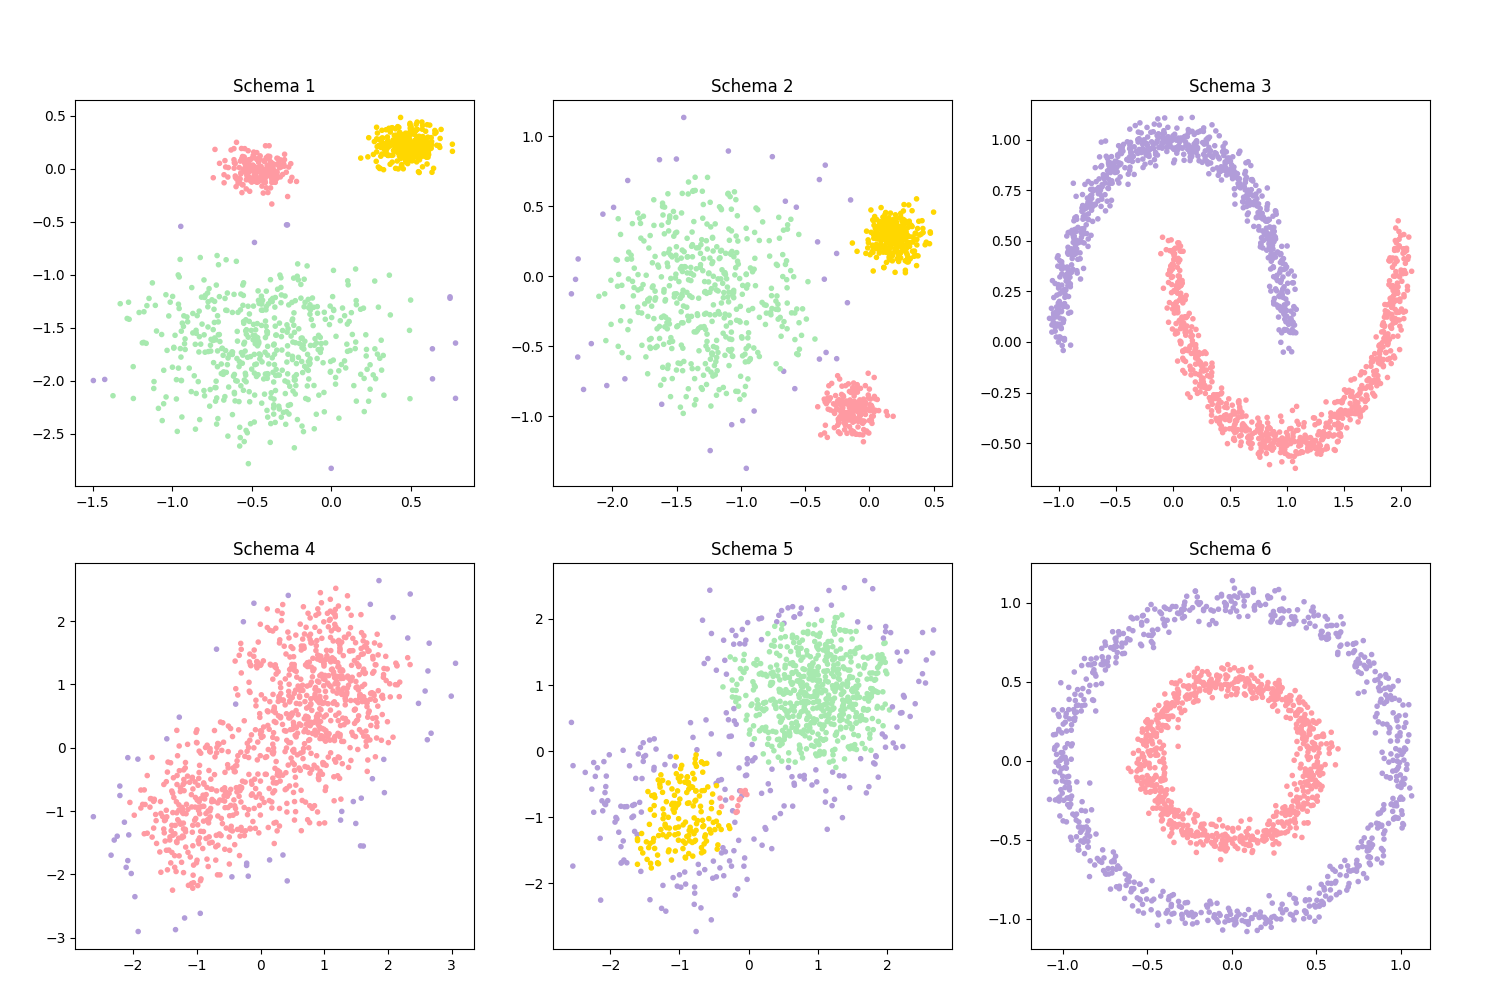
\includegraphics{src/memoire-umons/images/new_versions/dbscan_all.png}
\caption{Résultats de DBSCAN sur les bases de données
\label{dbscan_all}}
\end{figure}

\textbf{Evaluation de la performance DBSCAN vs CLARANS}

Dans l'article de Ester et al.\footfullcite{ester}, ils ont implémenté
DBSCAN en C++ en se basant sur une implémentation de l'arbre R*-tree,
ainsi que les stations de travail HP 735/100 ont été utilisé pour les
expériences. Une base de données du benchmark SEQUOI2A000 utilisée pour
l'expérience, représente un ensemble de données réelles des tâches en
sciences de la Terre, des sites californiens, issues du système
d'information sur les noms géographiques de l'US Geological Survey.

Étant donné la durée d'exécution élevée de CLARANS sur l'ensemble de
données, une partie de cette base de données est utilisée partiellement,
représentant entre 2\% et 20\% de l'ensemble complet.

Les résultats des expériences montrent, comme représentées à la figure
\ref{time}, provient de l'article de Ester et al.\footfullcite{ester},
que le temps d'exécution de DBSCAN augmente légèrement de manière
linéaire en fonction du nombre de points. Cela confirme que le temps
d'exécution de DBSCAN est de l'ordre de \(\mathcal{O}(n\cdot \log(n))\).
En revanche, le temps d'exécution de CLARANS présente une croissance
proche de la quadratique en fonction du nombre de points. DBSCAN
surpasse CLARANS d'un facteur compris entre 250 et 1900, cette
différence augmentant avec la taille de la base de données.

\begin{figure}
\centering
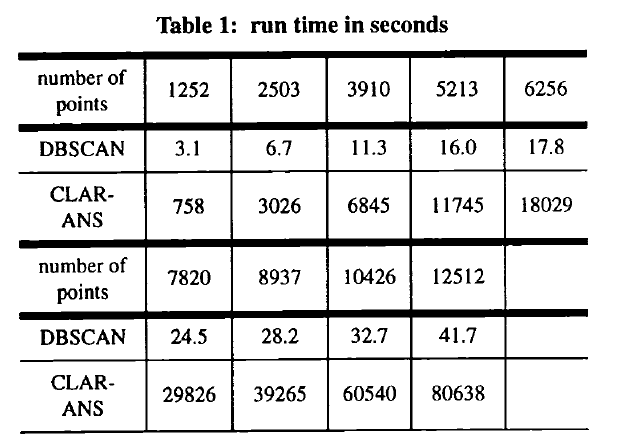
\includegraphics{src/memoire-umons/images/clarans_vs_dbscan.png}
\caption{Temps d'exécution CLARANS vs DBSCAN \label{time}}
\end{figure}

\chapter{Conclusion}

En conclusion, nous avons exploré en détail l'algorithme DBSCAN, une
méthode puissante de clustering basée sur la densité. Nous avons
souligné l'importance de choisir judicieusement les paramètres d'entrée,
tels que MinPts et Eps, pour garantir des résultats de clustering
optimaux. La sélection appropriée de ces paramètres est cruciale pour
obtenir une partition précise et significative des données.

Le modèle de HDBSCAN permet quant à lui de pouvoir pallier le problème
que DBSCAN fait face avec la création de ces clusters.

De plus, nous avons réalisé une comparaison approfondie entre DBSCAN et
CLARANS, mettant en évidence leurs performances respectives dans la
détection de clusters. Nos expériences ont démontré que DBSCAN est
capable de gérer des formes de clusters arbitraires et de détecter des
clusters de tailles différentes, ce qui le rend adapté à un large
éventail d'applications. En revanche, CLARANS a montré des performances
inférieures en termes de précision et de gestion des données bruitées.

Un autre aspect à prendre en compte est la complexité des deux
algorithmes. DBSCAN a une complexité temporelle de l'ordre de O(n log
n), tandis que CLARANS a une complexité quadratique, ce qui peut
entraîner des temps d'exécution significativement plus longs pour des
ensembles de données volumineux.

En conclusion, DBSCAN se révèle être un choix prometteur pour la
détection de clusters, avec une flexibilité dans la forme et la taille
des clusters identifiés. La sélection adéquate des paramètres d'entrée
et la compréhension des différences de performances entre DBSCAN et
CLARANS sont des éléments essentiels pour obtenir des résultats fiables
dans les applications de clustering.

\printbibliography[title=Bibliographie]

\end{document}
